% !TeX spellcheck = en_US
\addscenariosection{1}{Cooperative Scenario}{Brothers in Arms}{\images/berserk.png}

\begin{multicols*}{2}

\textbf{Author:} Kolartastic

\textbf{Source:} \href{https://discord.com/channels/740870068178649108/1161571991732625468/threads/1164804609605390386}{Archon Studios Discord}

\textit{Fight together. Die together.}  % no-check-caps

\subsection*{\MakeUppercase{Scenario Length}}
This Scenario plays out over 12 Rounds.

\subsection*{\MakeUppercase{Player Setup}}
\textbf{Player Count:} 2vs2 Alliance.

\textbf{Starting Resources:} 20 \svg{gold}, 3 \svg{building_materials}, 1 \svg{valuables}

\textbf{Starting Income:} 10 \svg{gold}, 0 \svg{building_materials}, 0 \svg{valuables}

\textbf{Starting Units:}

\begin{itemize}
  \item A Few of the cheapest \bronze\ Units.
  \item A Few of the cheapest \silver\ Units.
\end{itemize}

\textbf{Town Buildings:} \bronze\ Dwelling

\textbf{Additional Starting bonus:}
Choose one:
\begin{itemize}
  \item Search(3) \svg{skill}
  \item Search(3) \svg{spellpower}
  \item Add a Few \bronze\ Units of the second highest Recruitment cost.
\end{itemize}

\textbf{Map Tile Pool:} Each player takes one random Far (II–III) Map Tile.

\subsection*{\MakeUppercase{Map Setup}}
Take the following Map Tiles and arrange them as shown in the Scenario map layout:

\begin{itemize}
  \item 4 × Starting (I) Map Tiles.
  \item 2 × Far (II–III) Map Tiles.
  \item 4 × Near (IV–V) Map Tiles.
  \item 3 × Center (VI–VII) Map Tiles.
\end{itemize}

\subsection*{\MakeUppercase{Victory Conditions}}
The game ends when one team has captured both enemy Starting Towns – \textit{That team wins the game} or at the end of Round 12. If no team has captured both enemy Starting Towns, one player from both teams engage in final Combat.

\subsection*{\MakeUppercase{Timed Events}}
\textbf{\nth{4} Round:}
\begin{itemize}
  \item Remove all Black Cubes from the Map.
\end{itemize}
\textbf{\nth{6} Round:}
\begin{itemize}
  \item All players may trade resources or artifacts with one other player.
\end{itemize}
\textbf{\nth{9} Round:}
\begin{itemize}
  \item Repeat event of Round 6.
\end{itemize}

\subsection*{\MakeUppercase{Additional Rules}}
\begin{itemize}
  \item If two Heroes from the same team are on adjacent Fields, they can freely trade resources, Units and Artifacts.
  \item \textbf{Dragon Utopia:} Gain one Neutral Dragon you defeated.
  \item \textbf{Grail Token:} \svg{hand} Limit is increased to 10.
\end{itemize}

\begin{center}
  \vspace*{\fill}
  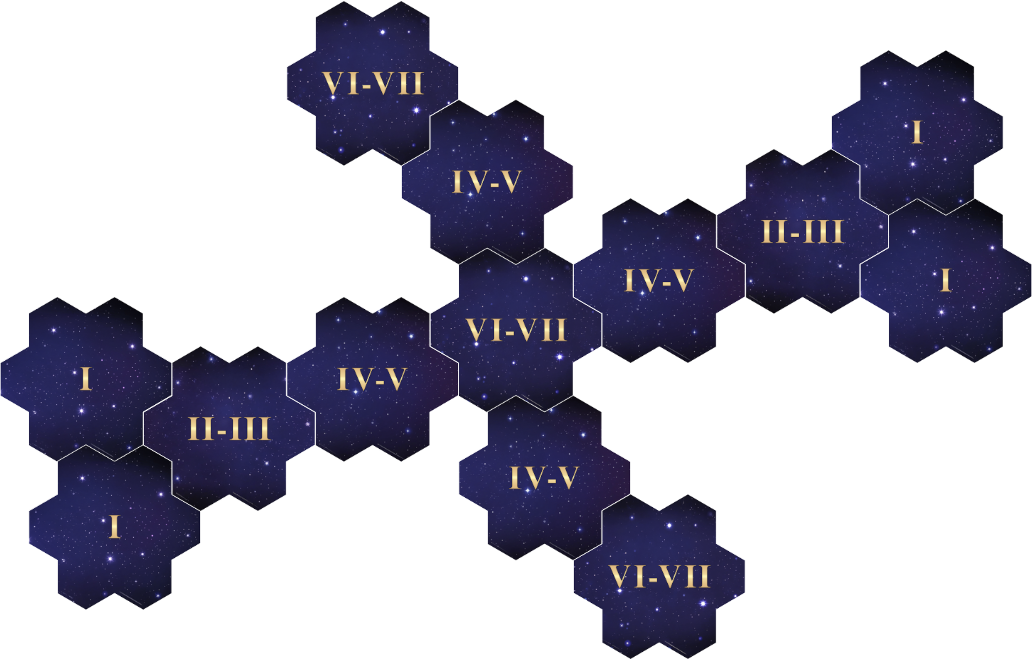
\includegraphics[width=0.7\linewidth]{\maps/brothers_in_arms.png}
  \captionof{figure}{\textbf{SCENARIO MAP LAYOUT}}
  \vspace*{\fill}
\end{center}
